\subsection{Word segmentation}
\label{sec:segmentation}



Does the model develop an implicit notion of word?
Early work on word segmentation suggests that high uncertainty about the next character \cite{cohen-algorithm-2001, feng-accessor-2004},  low transition probabilities \cite{harris-distributional-1954, saffran-word-1996} and low mutual information \cite{sun-chinese-1998} serve as statistical cues to word segmentation.
In Figure~\ref{fig:syntax-depth}, we plot (1) entropy of the predicted distribution over the net character around word boundaries, compared to other positions, and (2) the pointwise mutual information (PMI) between left and right contexts, computed by subtracting the unconditional likelihood of the next 20 characters from their likelihood conditioned on the prior context, both computed by the CNLM on a section of the German training set.
In accordance with prior work, higher entropy and lower PMI correlate with boundaries.


\begin{figure}
	\begin{center}
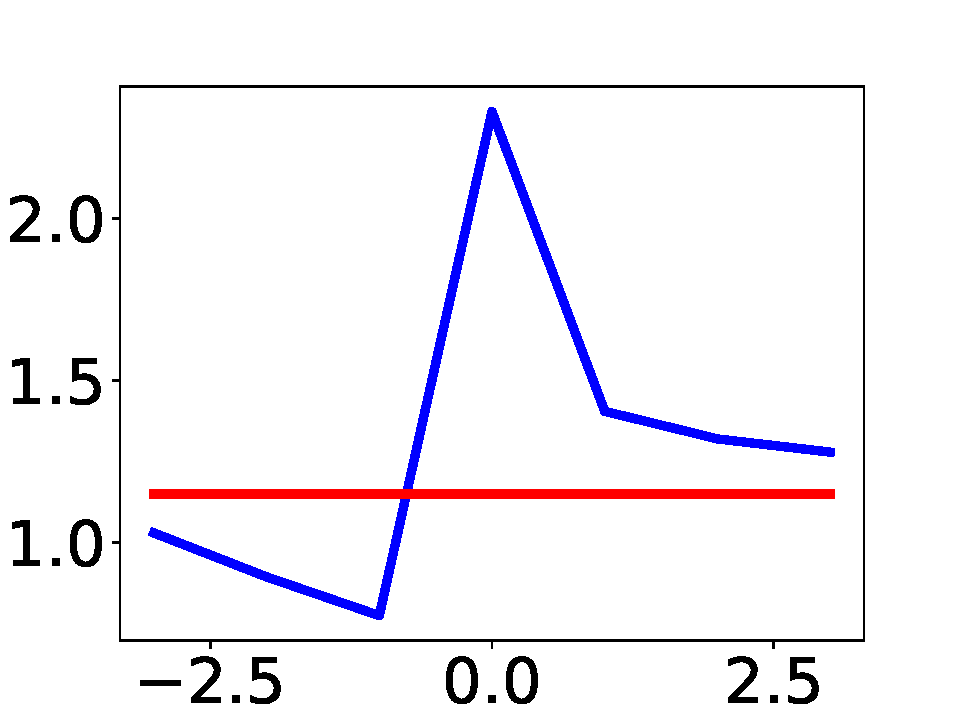
\includegraphics[width=0.22\textwidth]{figures/segmentation-profile-flattened-entropies-english.pdf}
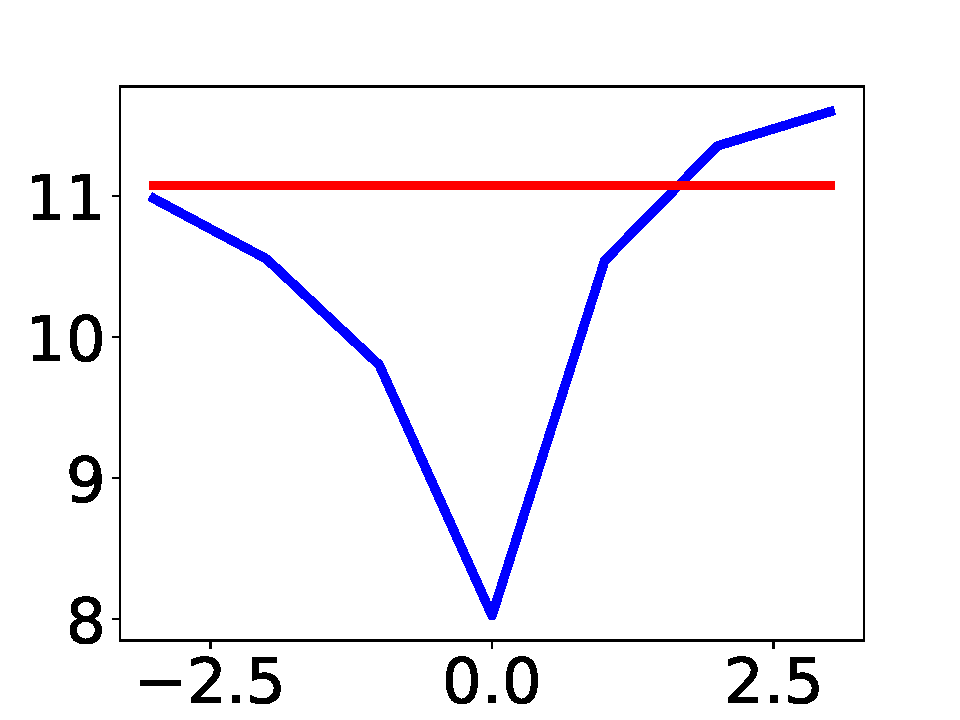
\includegraphics[width=0.22\textwidth]{figures/segmentation-profile-flattened-pmis-english.pdf}
	\end{center}
	\caption{Entropy over the next character (left) and PMI between left and right contexts (right) around word boundaries (blue); the x-axis indicates position relative to a word boundary. The red line indicates the overall average of the quantity. }\label{fig:boundaries-entropy}
\end{figure}


How reliable are these statistical cues, when computed by the CNLM?
We constructed a logistic regression predicting whether a character was the first one of a word or not, based on the following predictors:
(1) \emph{log-probability} of the character given prior context, (2) \emph{entropy} of the distribution over the character given prior context, (3) \emph{pmi of left and right contexts}, that is, the total likelihood of the next 20 characters, minus the unconditional likelihood estimated by starting the CNLM at the current position.
%The rationale of (3) is that it measures the pointwise mutual information, and thus the statistical association, between the subsequent characters and the prior context, which we hypothesize will be higher inside words.
%It is also the transition probability for the next characters
%(3) can also be interpreted as the result of normalizi transition probability
We collected these quantities for each position and for the preceding and following three characters.
%In total, the classifier has 21 coefficients.
We also conducted the same experiment with a character-level 8-gram model estimated on the training set, closer to the setup of earlier non-neural work.


\begin{table*}[t]
  \begin{center}
    \begin{tabular}{l|l|l|l|l}
      \multicolumn{1}{c}{}&\emph{LSTM}&\emph{RNN}&\emph{8-grams}\\
      \hline
      English & 65.83/60.37/62.98 &   63.26/59.81/61.49 & 55.73/51.0/53.26    \\ % \ldots{}/\ldots{}/\ldots & \ldots{}/\ldots{}/\ldots & \ldots{}/\ldots{}/\ldots &\ldots{}/\ldots{}/\ldots\\
      German &  57.012/52.505/54.67 &  53.2/49.26/51.15 & 42.89/36.28/39.31   \\ %   \ldots{}/\ldots{}/\ldots & \ldots{}/\ldots{}/\ldots & \ldots{}/\ldots{}/\ldots &\ldots{}/\ldots{}/\ldots\\
      Italian &  63.59/56.95/60.09 & 62.47/57.5/59.89  & 48.41/39.62/43.57    \\ % \ldots{}/\ldots{}/\ldots & \ldots{}/\ldots{}/\ldots & \ldots{}/\ldots{}/\ldots &\ldots{}/\ldots{}/\ldots\\
    \end{tabular}
  \end{center}
  \caption{\label{tab:segmentation-results} Precision recall, and F1 on word segmentation.}
\end{table*}

%PMI alone 
%P 30.56 R 20.61 F 24.61 German
%P 32.19 R 20.89 F 25.34 Italian
%P 39.37 R 29.45 F 33.69 English
%Surprisal alone
%P 28.04 R 18.64 F 22.4 German
%P 28.76 R 18.31 F 22.38 Italian
%P 33.65 R 24.1 F 28.08 English
%Entropy alone
%P 50.88 R 45.57 F 48.08 German
%P 58.44 R 52.09 F 55.08 Italian
%P 59.85 R 53.75 F 56.63 English


For each language model and language, we compute how many of the extracted tokens were correct (precision) and how many of the actual tokens were found by the classifier (recall), together with F1.
The goal of this experiment is not to construct a new word segmentation system, but to evaluate how strongly the CNLM's probabilities are indicative of word boundaries.

Results are shown in Figure~\ref{tab:segmentation-results}, showing that the CNLM-based classifiers robustly segment more than half of the tokens correctly, and do considerably better than the character 8-gram model.
Ablation shows that entropy is most predictive, reaching an F1 of 56.63 (English), 48.08 (German), 55.08 (Italian) alone.
Surprisal reaches 28.08 (English), 22.4 (German), 22.38 (Italian); PMI reaches 33.69 (English), 24.61 (German), 25.34 (Italian).
%Setting N to other values shows that larger values of N increase performance (N =10: 62.45, N=20: 63.24).

How does the LSTM CNLM compare to unsupervised word segmentation models?
We compare to the Bayesian bigram model of \cite{goldwater-bayesian-2009}, an elegant model using a hierarchical Dirichlet process.
Running Bayesian methods on the Wikipedia dumps is computationally infeasible; thus we also created a CNLM on the Brent corpus \cite{brent-efficient-1999} of child-directed speech.
We used 90 \% to train our language model, 5 \% to fit the logistic regression, and 5 \% to evaluate word segmentation.
(This compares with the Bayesian models that train and evaluate on the full dataset, but incorporate no word boundary information in their training signal).

\begin{table*}[t]
  \begin{center}
    \begin{tabular}{ll|l|l|l|l}
      \multicolumn{2}{c|}{}&Tokens & Lexical & Boundaries\\      \hline
	    \multirow{4}{*}{CNLM} & Full model & 0.75/0.76/0.75 & 0.41/0.61/0.49 & 0.91/0.90/0.90 \\
	    &     log-probability & 0.510/0.453/0.480 & 0.488/0.195/0.279 & 0.805/0.716/0.758 \\
	    &     entropy & 0.504/0.533/0.518 & 0.520/0.211/0.300 & 0.790/0.747/0.768\\
	    &     PMI & 0.708/0.729/0.718 & 0.576/0.346/0.432 &0.899/0.873/0.886  \\ \hline
	    \multicolumn{2}{c|}{\citet{goldwater-bayesian-2009}} & 0.752/0.696/0.723 & 0.635/0.552/0.591 & 0.903/0.808/0.852
    \end{tabular}
  \end{center}
	\caption{\label{tab:segmentation-results-brent} Word segmentation results on the Brent corpus for our model, for the three individual predictors, and the Bayesian model of \cite{goldwater-bayesian-2009}. Following \cite{goldwater-bayesian-2009}, we evaluate on the level of tokens, the lexicon of induced word types, and boundaries.}
\end{table*}

Results in Table~\ref{tab:segmentation-results-brent} show that the performance is broadly comparable to that of a sophisticated Bayesian segmentation method.
This suggests that statistical properties as modeled by the CNLM provide reliable cues to word boundaries.\footnote{We also created a logistic regression on hidden states, obtaining accuracy over 90 \% in classifying word boundaries on unseen words, outperforming an n-gram-count baseline. This suggests that the model internally tracks word boundaries.}
In contrast to the Wikipedia experiments, PMI emerges as the most important predictor on this dataset.

Unlike our method, the Bayesian method is fully unsupervised, but it has a built-in bias towards a discrete lexicon with a power-law frequency distribution.
Note that, unlike supervised word segmentation methods, our classifier does not have access to the character strings directly; instead, it evaluates how strongly quantities computed by the CNLM \emph{correlate} with word boundaries.



Looking at the main errors made by our English CNLM is instructive. We
consider first the 30 most common undersegmentations in the test set
(that is, cases in which the model failed to split two or more
words). About half (16) of them are common function word sequences
that could indeed easily be re-analyzed as single words (e.g.,
\emph{more than}, \emph{as well as}, \emph{such as}). Of the remaining
cases, 8 follow the \emph{N of} pattern, where \emph{N} is a
(typically relational) noun commonly occurring in this construction
(\emph{member of}, \emph{end of}, \emph{part of}\ldots). There are 3
fixed multi-word expressions (\emph{New York}, \emph{United States}
and \emph{high school}). Finally, it's reasonable to treat \emph{based
  on}, \emph{known as} and \emph{according to} as lexicalized
connectives, especially in the Wikipedia text the model was trained
upon.

The picture is a bit murkier but still fairly linguistically grounded
for the 30 most common oversegmentation errors (that is, the character
fragments that are wrongly segmented from inside the largest number of
distinct words).\footnote{We ignore here single-letter segmentations,
  that would otherwise account for one third of the most-frequent
  set.}  More than half (17) are common affixes (prefixes such as
\emph{re} and \emph{de} or suffixes such as \emph{ing} and
\emph{ly}). The remaining cases include 3 strings identical to frequent
function words wrongly carved out of longer words (\emph{the},
\emph{to} and \emph{on}, although the model might be treating the
latter as a pseudo-suffix in forms such as \emph{Peterson} and
\emph{Creighton}). Further, the strings \emph{land} and \emph{man} are not
unreasonably segmented out of compounds. It's hard, on the other hand,
to find a linguistically sound motivation for the 8 remaining top
oversegmentations (\emph{la, le, ma, na, ra, ro, se, ta}).

We hypothesized that similar statistical correlates exist for hierarchical syntactic structure.
We created constituency trees for the German validation set using the Berkeley Parser~\ref{petrov2007improved}.
For each character in the data, we counted its hierarchical distance from the preceding character, operationalized as the number of intervening closing and opening brackets.
This number is zero if and only if both characters belong to the same word.

Figure~\ref{fig:syntax-depth} plots PMI by hierarchical ditance.
The plot shows that longer hierarchical distance between neighboring characters corresponds to lower average MI, generalizing the finding for word boundaries.
This illustrates how it is useful for segmentation knowledge to be implicit, as the model ``knows'' about different kinds of boundaries in a continuous manner.

\begin{figure}
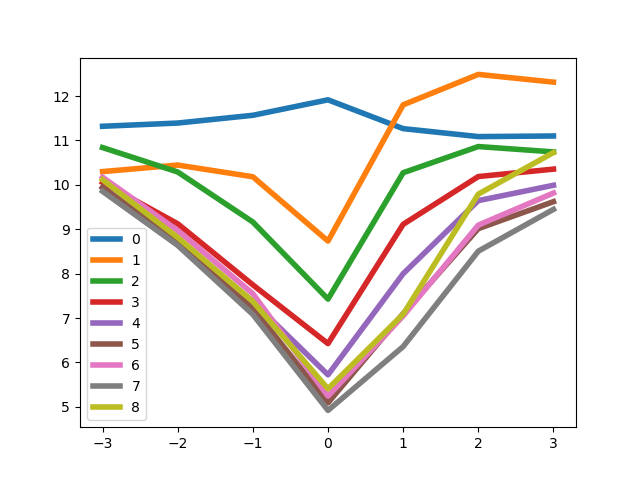
\includegraphics[width=0.48\textwidth]{figures/segmentation-profile-pmis-german-all-heights.png}
\caption{PMI between left and right contexts, estimated by the CNLM, by syntactic hierarchical distance between subsequent characters.}\label{fig:syntax-depth}
\end{figure}


